\documentclass{article}

% if you need to pass options to natbib, use, e.g.:
%     \PassOptionsToPackage{numbers, compress}{natbib}
% before loading neurips_2018

% ready for submission
% \usepackage{neurips_2018}

% to compile a preprint version, e.g., for submission to arXiv, add add the
% [preprint] option:
%     \usepackage[preprint]{neurips_2018}

% to compile a camera-ready version, add the [final] option, e.g.:
     \usepackage[final]{neurips_2018}

% to avoid loading the natbib package, add option nonatbib:
%     \usepackage[nonatbib]{neurips_2018}

\usepackage[utf8]{inputenc} % allow utf-8 input
\usepackage[T1]{fontenc}    % use 8-bit T1 fonts
\usepackage{hyperref}       % hyperlinks
\usepackage{url}            % simple URL typesetting
\usepackage{booktabs}       % professional-quality tables
\usepackage{amsfonts}       % blackboard math symbols
\usepackage{nicefrac}       % compact symbols for 1/2, etc.
\usepackage{microtype}      % microtypography
\usepackage{graphicx}
\usepackage{caption}
\usepackage{subcaption}
\usepackage{float}
\usepackage{setspace}
\usepackage{amsmath}
\onehalfspacing
\title{Neural Networks as Universal Function Approximators and Exponential Advantage of Deep Networks Over Shallow Networks}

% The \author macro works with any number of authors. There are two commands
% used to separate the names and addresses of multiple authors: \And and \AND.
%
% Using \And between authors leaves it to LaTeX to determine where to break the
% lines. Using \AND forces a line break at that point. So, if LaTeX puts 3 of 4
% authors names on the first line, and the last on the second line, try using
% \AND instead of \And before the third author name.

\author{%
  Muhammad Usaid \\
  Department of Computer Science\\
  Dhanani School of Science and Engineering \\
  Habib University\\
  \texttt{mu04032@st.habib.edu.pk}
  \And 
  Muhammad Munawwar \\
  Department of Computer Science\\
  Dhanani School of Science and Engineering \\
  Habib University\\
  \texttt{ma04289@st.habib.edu.pk}
  \And 
  Khubaib Naeem \\
  Department of Computer Science\\
    Dhanani School of Science and Engineering \\
    Habib University\\
  \texttt{kk04333@st.habib.edu.pk}
  % examples of more authors
  % \And
  % Coauthor \\
  % Affiliation \\
  % Address \\
  % \texttt{email} \\
  % \AND
  % Coauthor \\
  % Affiliation \\
  % Address \\
  % \texttt{email} \\
  % \And
  % Coauthor \\
  % Affiliation \\
  % Address \\
  % \texttt{email} \\
  % \And
  % Coauthor \\
  % Affiliation \\
  % Address \\
  % \texttt{email} \\
}

\begin{document}
% \nipsfinalcopy is no longer used

\maketitle

\begin{abstract}
    The idea regarding the power of neural networks to approximate any function has been around for a while. We have seen theoretical results since 1989 that under certain assumptions, a neural network with single layer can approximate any function. In this report we will dive into this idea by analyzing a theorem and it's proof regarding approximating a multivariate polynomial with a neural network. We will further discuss the inefficiency of neural networks with one hidden layer in terms of minimum number of neurons required to approximate a monomial and will see the upper and lower bounds on minimum number of neurons required in one hidden layer and a deep network. We will see how going deep and adding more layers gives exponential advantage and increases with the logarithm of number of inputs unlike shallow network. We have also provided some visual proves which is a good way to understand what's going on in the networks. We will see what functions and shapes we can plot by changing the parameters of the neural network.
\end{abstract}

\section{Introduction}
Deep Learning has shown amazing progress in last two decades with us being able to classify images, translating languages, detecting objects with a camera and so many other useful applications. But still deep learning networks are something that are not completely understood. People have been working on understanding neural networks theoretically and coming up with theorems and bounds on the power of neural networks as universal function approximators. Since then there have been different results on how much neural networks can do by making some reasonable assumptions. We will explore this area with some visualizations on the way. We will shed light on some theorems that gives us the bounds on the minimum number of neurons required in deep and shallow networks.

\section{Literature Review}
The first kind of work that has been done in this field in 1989 was by Cybenko \cite{paper1989_1} in which he showed how to approximate functions by the superposition of a sigmoidal function and by Funahashi \cite{paper1989_2} in which he showed some results for approximation of continuous mappings by neural networks. Hornit at el. \cite{paper1989_3} showed that multilayer feed forward networks are able to approximate any Borel measurable function from one finite dimensional space to another to any desired degree of accuracy. Barron \cite{paper1994} showed approximation and estimation bounds on artificial neural networks. Pinku \cite{paper1999} showed some approximation-theoretic problems that arise in the multilayer feedforward perceptron (MLP) model in neural networks and discussed them mathematically.
\section{Neural networks as universal approximators}
\subsection{Neural networks can compute any function}
The universality theorem of neural networks also applies when the function has multiple inputs and outputs. Moreover, this result is true if we add a constraint of just one hidden layer. The universality theorem of neural networks implies that they can compute any function \cite{website1}. This statement needs to be quantified further. Firstly, Neural networks cannot exactly compute any function, instead they approximate the function. Secondly, if the function is discontinuous, neural networks cannot be used to approximate the function. This is because the neural networks compute a continuous function of their input. However, neural networks can compute a continuous approximation for a discontinuous function. Consequently, we can define neural networks as universal approximators which can approximate any continuous function to any given precision.


\subsection{Approximating multivariate polynomials with k-layer networks \cite{paper1}}
Neural networks are extremely powerful and can approximate multivariate polynomials. It can be considered its own multivariate function $N(x) = A_k \sigma(A_{k-1} \sigma(\cdots \sigma(A_1x \sigma (A_0x))\dots)$, where $A_0,A_1,\dots A_k$ are constant matrices and our activation function $\sigma$, is a nonlinear function that is applied element-wise to vectors. $k$ is referred to as the depth of the network. The neurons of the network are the entries of the vectors $\sigma(A_l \dots \sigma A_1(\sigma (A_0 x)\dots)$ for $l=1,\dots, k-1$. These vectors are hidden layers of the network. \\
In order to prove that that we can approximate multivariate polynomials using neural networks, we need the following definitions for approximating multivariate functions: \\
\textbf{$\mathbf{\epsilon}$-approximation / uniform approximation} For constant $\epsilon>0$, we say that a network $N(x)$ $\epsilon$ approximates a multivariate function $f(x)$ for a $x$ in a specified domain $(-R,R)^n$ if $\sup_{x} |N(x)-f(x)|<\epsilon$ \\
\textbf{Taylor approximation}: A network $N(x)$ Taylor approximates a multivariate polynomial $p(x)$ of degree $d$ if $p(x)$ is the $d$th order Taylor polynomial of $N(x)$ at about the origin. \\
If we can Taylor approximate a homogeneous polynomial, then we can also $\epsilon$-approximate that polynomial. This can be represented as a proposition. \\
\textbf{Proposition:} Suppose that the network $N(x)$ Taylor approximates the homogeneous multivariate polynomial $p(x)$, then for every $\epsilon$, there exists a network $N_{\epsilon}(x)$ that $\epsilon$- approximates $p(x)$ (for any specified domain $x \in (-R,R)^n$ for any specified $R$) such that $N(x)$ and $N_{\epsilon}(x)$ have the same number of neurons in each layer. 
\\
\textbf{Proof:} Suppose that $N(x) = A_k \sigma(A_{k-1} \sigma(\cdots \sigma (A_0x)\dots)$ and that $p(x)$ has degree $d$. Since $p(x)$ is a taylor approximation of $N(x)$ we can write $N(x)$ as $p(x) + E(x)$, where $E(x) = \sum_{i=d+1}^{\infty}E_i(x)$ is a taylor series with each $E_i(x)$ homogenous of degree $i$. Since $N(x)$ is the function defined by a neural network, it converges for every $x \in \mathbb{R}^n$. Thus, $E(x)$ converges, as does $E(\delta x)/\delta^d = \sum_{i=d+1}^{\infty}\delta^{i-d}E_i(x)$. By picking $\delta$ sufficiently small, we can make each term $\delta^{i-d}E_i(x)$. Let $\delta$ be small enough that $|E(\delta x)/\delta^d|<\epsilon$. \\
Let $A_0^{'} = \delta A_0, A_k^{'} = A^{k} / \delta^d $ 
and $A_{l}^{i} = A_l$ for $l =1,\dots,k-1.$ Then for $N_{\epsilon}(x) = A_k^{'} \sigma(\dots \sigma(A_1^{'} \delta (A_0^{'} x)) \dots )$ we observe that $N_{\epsilon}(x) = N(\delta x)/\sigma^d$ and therefore 
$$|N_{\epsilon}(x) - p(x)| = |N(\delta x)/\delta^d -p(x)| $$
$$= |p(\delta x)/\delta^d + E(\delta x)/\delta^d - p(x)|$$
$$= |E(\delta x)/\delta^d|< \epsilon$$
Hence $N_{\epsilon}(x)$ is an $\epsilon$ approximation of $p(x)$ as desired.
% Proof daalo if time
\subsubsection{Theorem}
Suppose that $p(x)$ is a degree $d$ multivariate polynomial and the non linearity $\sigma$ has nonzero taylor coefficients up to the degree $d$. Let $m_k^{\epsilon}(p)$ be the minimum number of neurons in a depth $k$ network that $\epsilon$-approximates $p$. The the limit $\lim_{\epsilon \to 0} m_k^{\epsilon}(p)$ exists and is finite. (for $x \in (-R,R)^n$ for any specified $R$). \\
\textbf{Proof:} We show that $\lim_{\epsilon \to 0} m_1^{\epsilon} (p)$ exists then $\lim_{\epsilon \to 0} m_k^{\epsilon} (p)$ exists for every $k$ since an $\epsilon$ approximation to $p(x)$ with depth $k$ can be constructed from depth 1. 
\\Let $p_1(x),p_2(x),\dots,p_s(x)$ be the monomials of $p(x)$ so that $p(x) = \sum_i p_i(x)$. Using the proof from Lin et al \cite{lin2017},
we know that products can be taylor approximated by networks with one hidden layer hence, therefore since each monomial is the product of several inputs (with multiplicity) we can taylor approximate each $p_i(x)$ by a network $N^i(x)$ with one hidden layer. \\
Suppose now that $N^i(x)$ has hidden $m_i$ neurons. By our proposition, since $p_i(x)$ is homogeneous, it may be $\delta$-approximated by a network $N_{\delta}^i(x)$ for each $i$. We can now define a network $N_{\epsilon}(x) = \sum_{i} N_{\delta}^{i}(x)$ with $\sum_i m_i$ neurons. This network does indeed $\epsilon$-approximate since:
$$|N_{\epsilon}(x) - p(x)|\leq \sum_i |N_{\delta}^{i} (x) - p_i(x)|$$
$$\leq \sum_i \delta = s\delta = \epsilon$$
This implies that $m_1^{\epsilon} (p) \leq \sum_i m_i$ neurons for every $\epsilon$. Thus $\lim_{\epsilon \to 0} m_1^{\epsilon} (p)$ exists.\\
% Bolon ke relu kaam nahi kare ga?





\section{The Efficiency of Deep Networks over Shallow Networks}
This section deals with the discussion related to the performance of deep and shallow networks where shallow means the network with just one hidden layer. The first two theorems will show the result for uniform and Taylor approximation of a monomial with a neural network and we will see that shallow networks requires exponentially greater neurons than deep network to approximate the monomial.
\subsection{Theorem}
Let $p(x)$ denote the monomial ${x_1}^{r_1} {x_2}^{r_2} {x_3}^{r_3} ...$ ${x_n}^{r_n}$ with $d=\sum\limits_{i=1}^n r_i$. Suppose that the nonlinearity $\sigma$ has nonzero Taylor coefficients up to degree $2d$ \cite{paper1}. Then, we have:
    \begin{itemize}
        \item $m_1^{\text{uniform}} (p) = \prod\limits_{i=1}^n (r_i + 1)$
        \item $m^{\text{uniform}} (p) \leq \sum\limits_{i=1}^n (7 \lceil \log_2 (r_i) \rceil + 4)$ 
    \end{itemize}
Here the uniform approximation is the $\epsilon$-approximation that we talked about earlier. $m_1^{\text{uniform}}(p)$ means the minimum number of neurons in a network with one layer to approximate the polynomial $p$. Meanwhile $m^{\text{uniform}} (p)$ means the minimum number of neurons in deep network required to approximate the polynomial $p$.
\subsection{Theorem}
Let $p(x)$ denote the monomial ${x_1}^{r_1} {x_2}^{r_2} {x_3}^{r_3} ...$ ${x_n}^{r_n}$ with $d=\sum\limits_{i=1}^n r_i$. Suppose that the nonlinearity $\sigma$ has nonzero Taylor coefficients up to degree $d$ \cite{paper1}. Then, we have:
    \begin{itemize}
        \item $m_1^{\text{Taylor}} (p) = \prod\limits_{i=1}^n (r_i + 1)$
        \item $m^{\text{Taylor}} (p) \leq \sum\limits_{i=1}^n (7 \lceil \log_2 (r_i) \rceil + 4)$
    \end{itemize}

This is the same thing as in previous theorem with just one change that it is for Taylor approximation. One thing to notice here is that these two theorems does not imply each other. We can see that in deep networks, we are taking the logarithm of the powers so it will be exponentially better than shallow networks when we increase the number of variables in the monomial. 
\subsection{Experimentation}
Let's try to understand these theorems by doing some maths and using some examples. Suppose we have a monomial $\prod_i{x_i}^4$ and compare the minimum number of neurons in deep and shallow network according to the formula we just saw in theorems. We can see the results in Table \ref{table1}. We can also have a better look visually by plotting it on the graph. The graph can be seen in Figure \ref{fig:figure1}.
\begin{center}
    \begin{table}[H]
        \centering
        \begin{tabular}{|c|c|c|}
        \hline
        Monomial & Min Neurons in 1 layer & Min Neurons in Deep Network \\
        \hline
            ${x_1}^4 {x_2}^4 ... {x_n}^4$ & $\prod\limits_{i=1}^n (r_i + 1)$ & $\sum\limits_{i=1}^n (7 \lceil \log_2 (r_i) \rceil + 4)$\\
        \hline
        ${x_1}^4$ & 5 & 18\\
        \hline
        ${x_1}^4 {x_2}^4$ & 25 & 36\\
        \hline
        ${x_1}^4 {x_2}^4 {x_3}^4$ & 125 & 54\\
        \hline
        ${x_1}^4 {x_2}^4 {x_3}^4 {x_4}^4$ & 625 & 72\\
        \hline
        ${x_1}^4 {x_2}^4 {x_3}^4 {x_4}^4 {x_5}^4$ & 3125 & 90\\
        \hline
        ${x_1}^4 {x_2}^4 {x_3}^4 {x_4}^4 {x_5}^4 {x_6}^4$ & 15625 & 108\\
        \hline
        \end{tabular}
        \caption{Comparison of minimum number of neurons}
        \label{table1}
    \end{table}
    \end{center}
% \newpage
\begin{figure}[H]
    \centering
    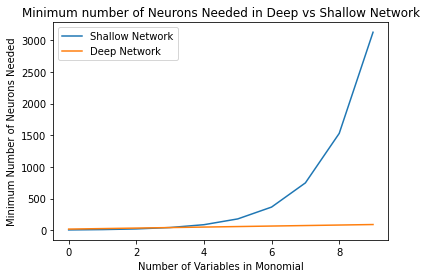
\includegraphics[width=0.8 \textwidth]{Images/comparison.jpg}
    \caption{Graph of deep vs shallow network for neurons}
    \label{fig:figure1}
\end{figure}

Let consider an example of Theorem 4.1 . Let $f(x,y) = x^8 y^8$. See Figure \ref{fig:figure20}. The values of the parameters were 
\begin{itemize}
    \item Number of Epochs = 500
    \item Batch Size = 20
    \item Optimizer algorithm = Adam
    \item activation function = Tanh
\end{itemize}
\begin{figure}[h!]
    \centering
    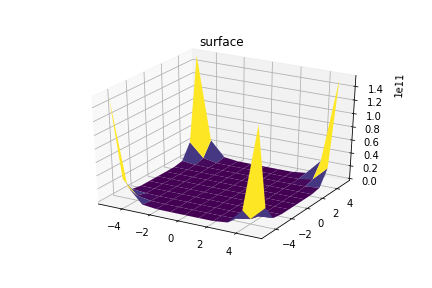
\includegraphics[width=0.7 \textwidth]{Images/1/Original.png}
    \caption{$f(x,y) = x^8 y^8$}
    \label{fig:figure20}
\end{figure}
\newpage
If we are using a single hidden layer, then minimum number of neurons that are required are $ 81 = 9 \times 9 $. The shallow network approximated $f(x)$ with $ \mbox{MSE} = 0.06$
\begin{figure}[h!]
    \centering
    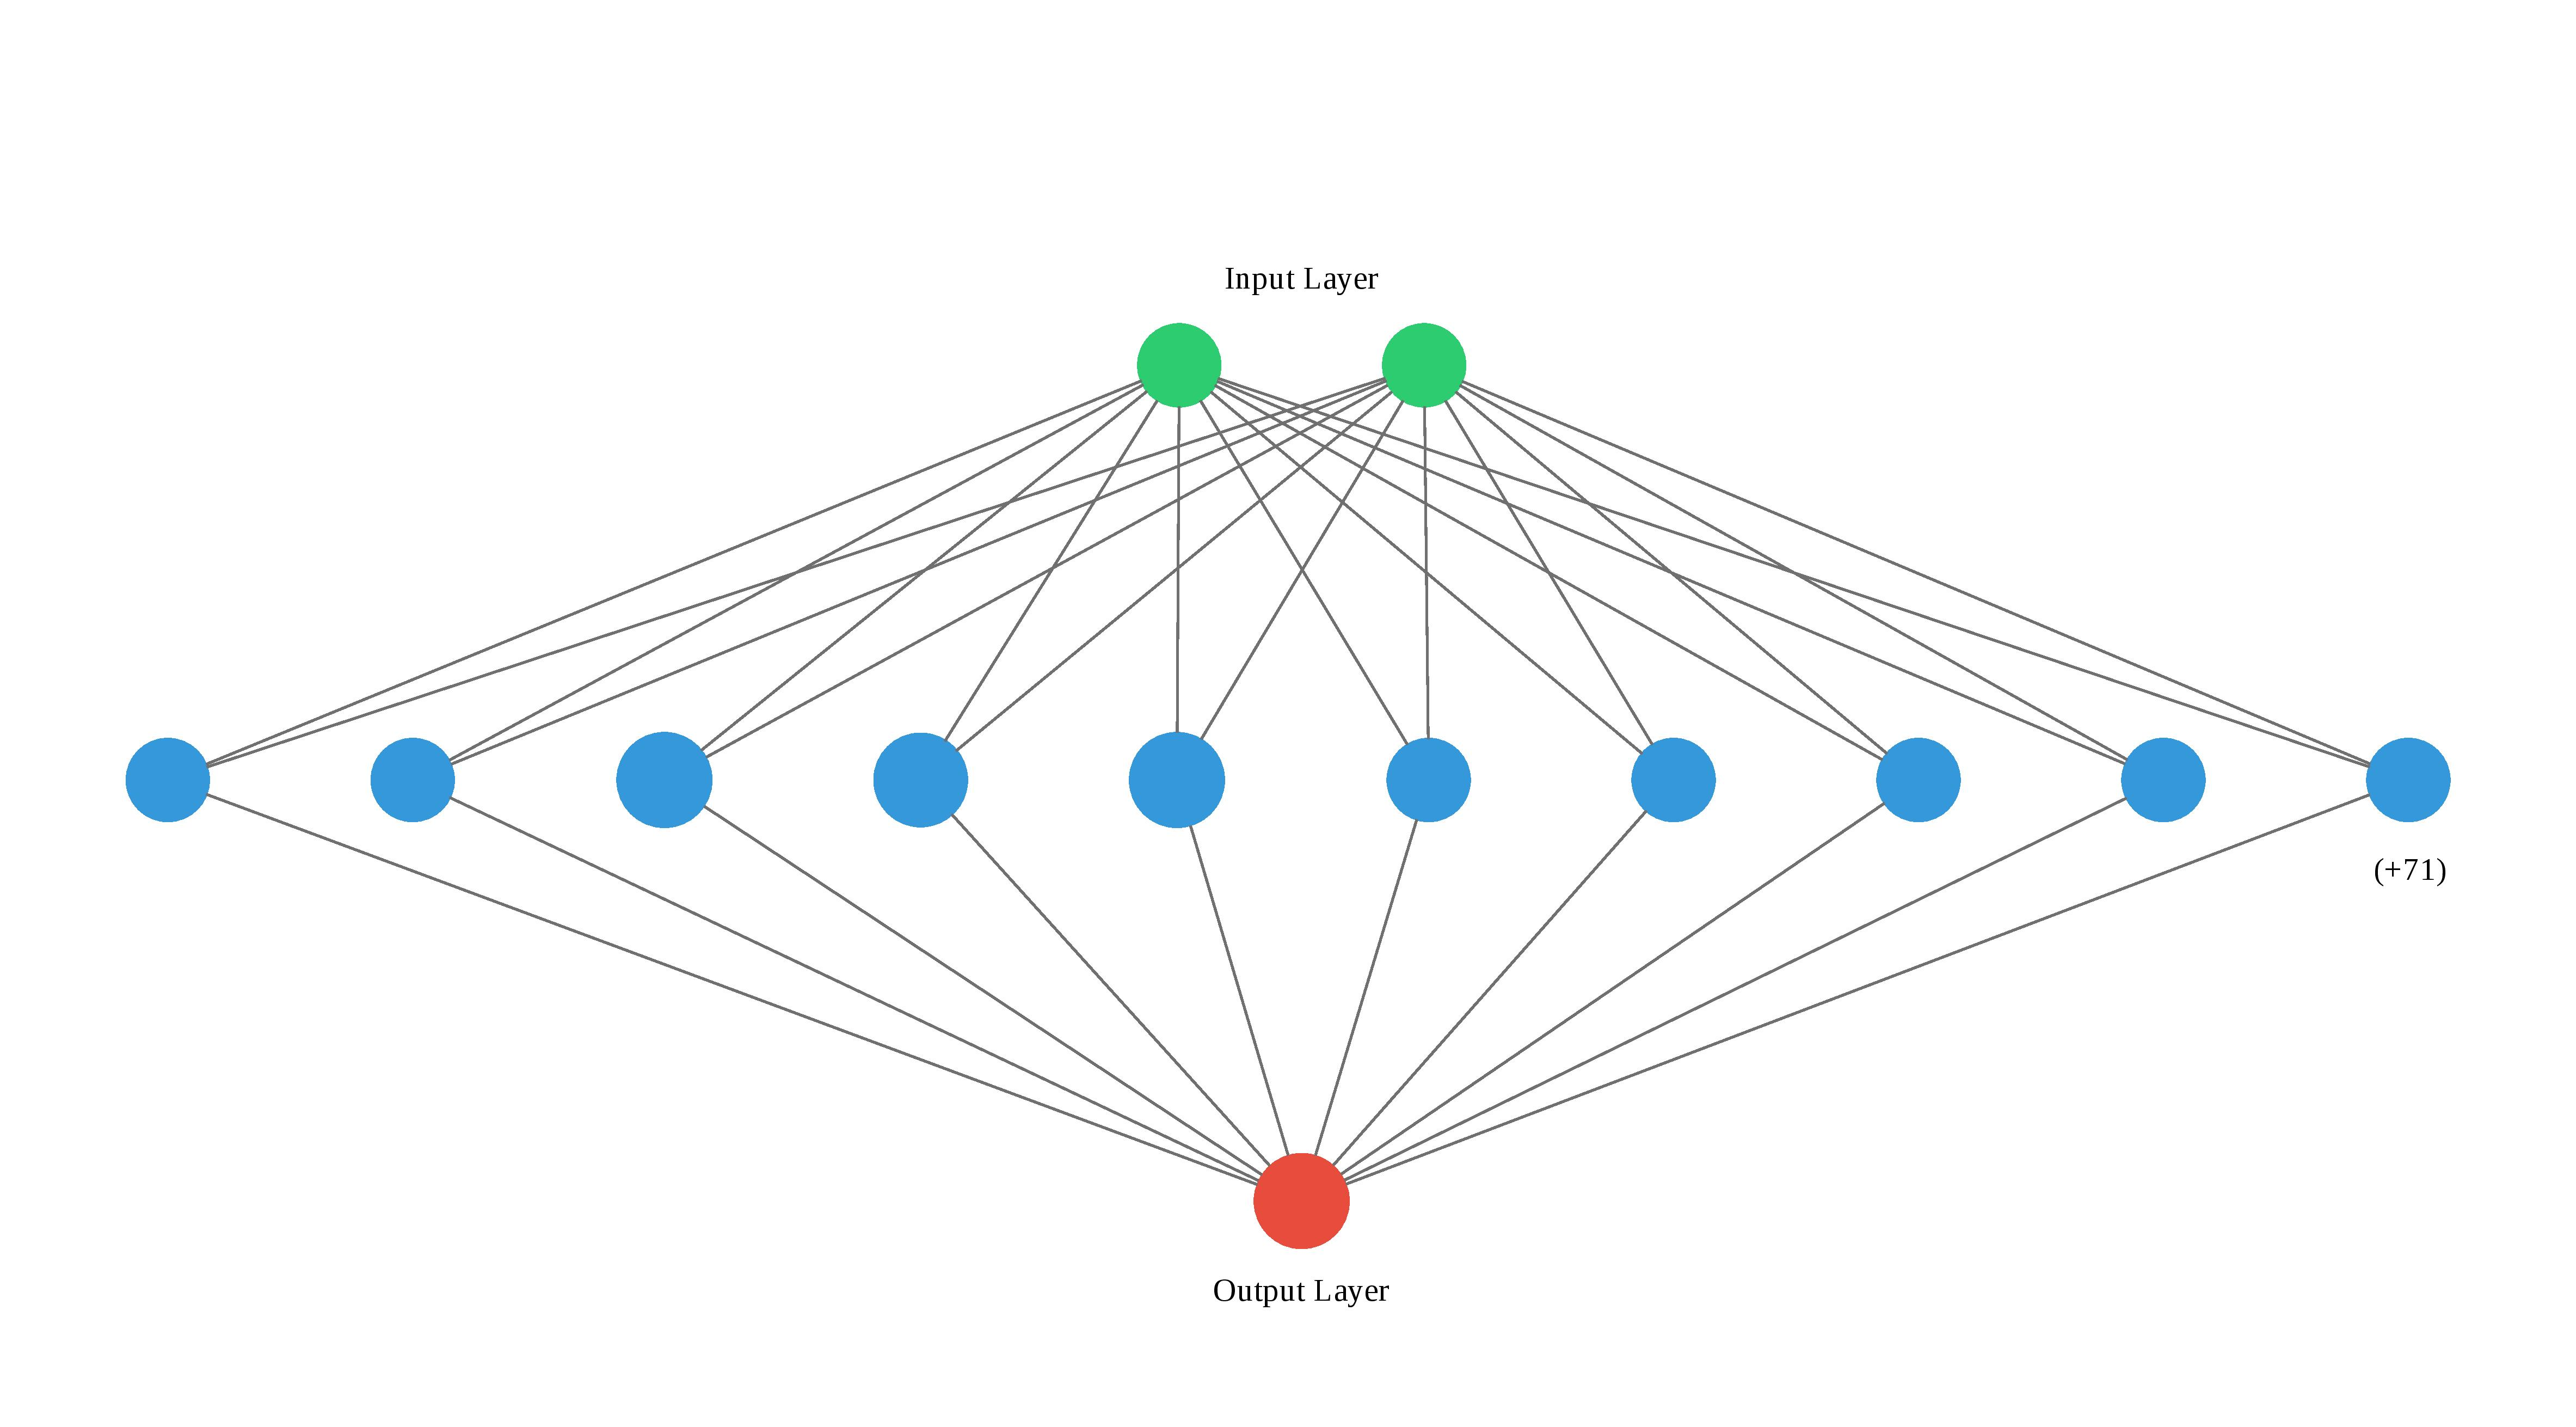
\includegraphics[width=0.8 \textwidth]{Images/1/ShallowNetwork81.jpg}
    \caption{Single Hidden Layer with 81 neurons}
    \label{fig:figure21}
\end{figure}

\begin{figure}[h!]
    \centering
    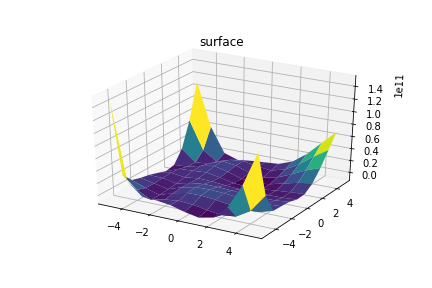
\includegraphics[width=0.8 \textwidth]{Images/1/PredictShallow.png}
    \caption{Approximation of $f(x)$ with MSE 0.06}
    \label{fig:figure22}
\end{figure}
\newpage
If we are using two hidden layer, then minimum number of neurons that are required are $ 25 $. The deep network approximated f(x) with $\mbox{MSE} = 0.00$. Hence, a deep network with a fewer number of total neurons than shallow networks was able to better approximate $f(x)$.
\begin{figure}[h!]
    \centering
    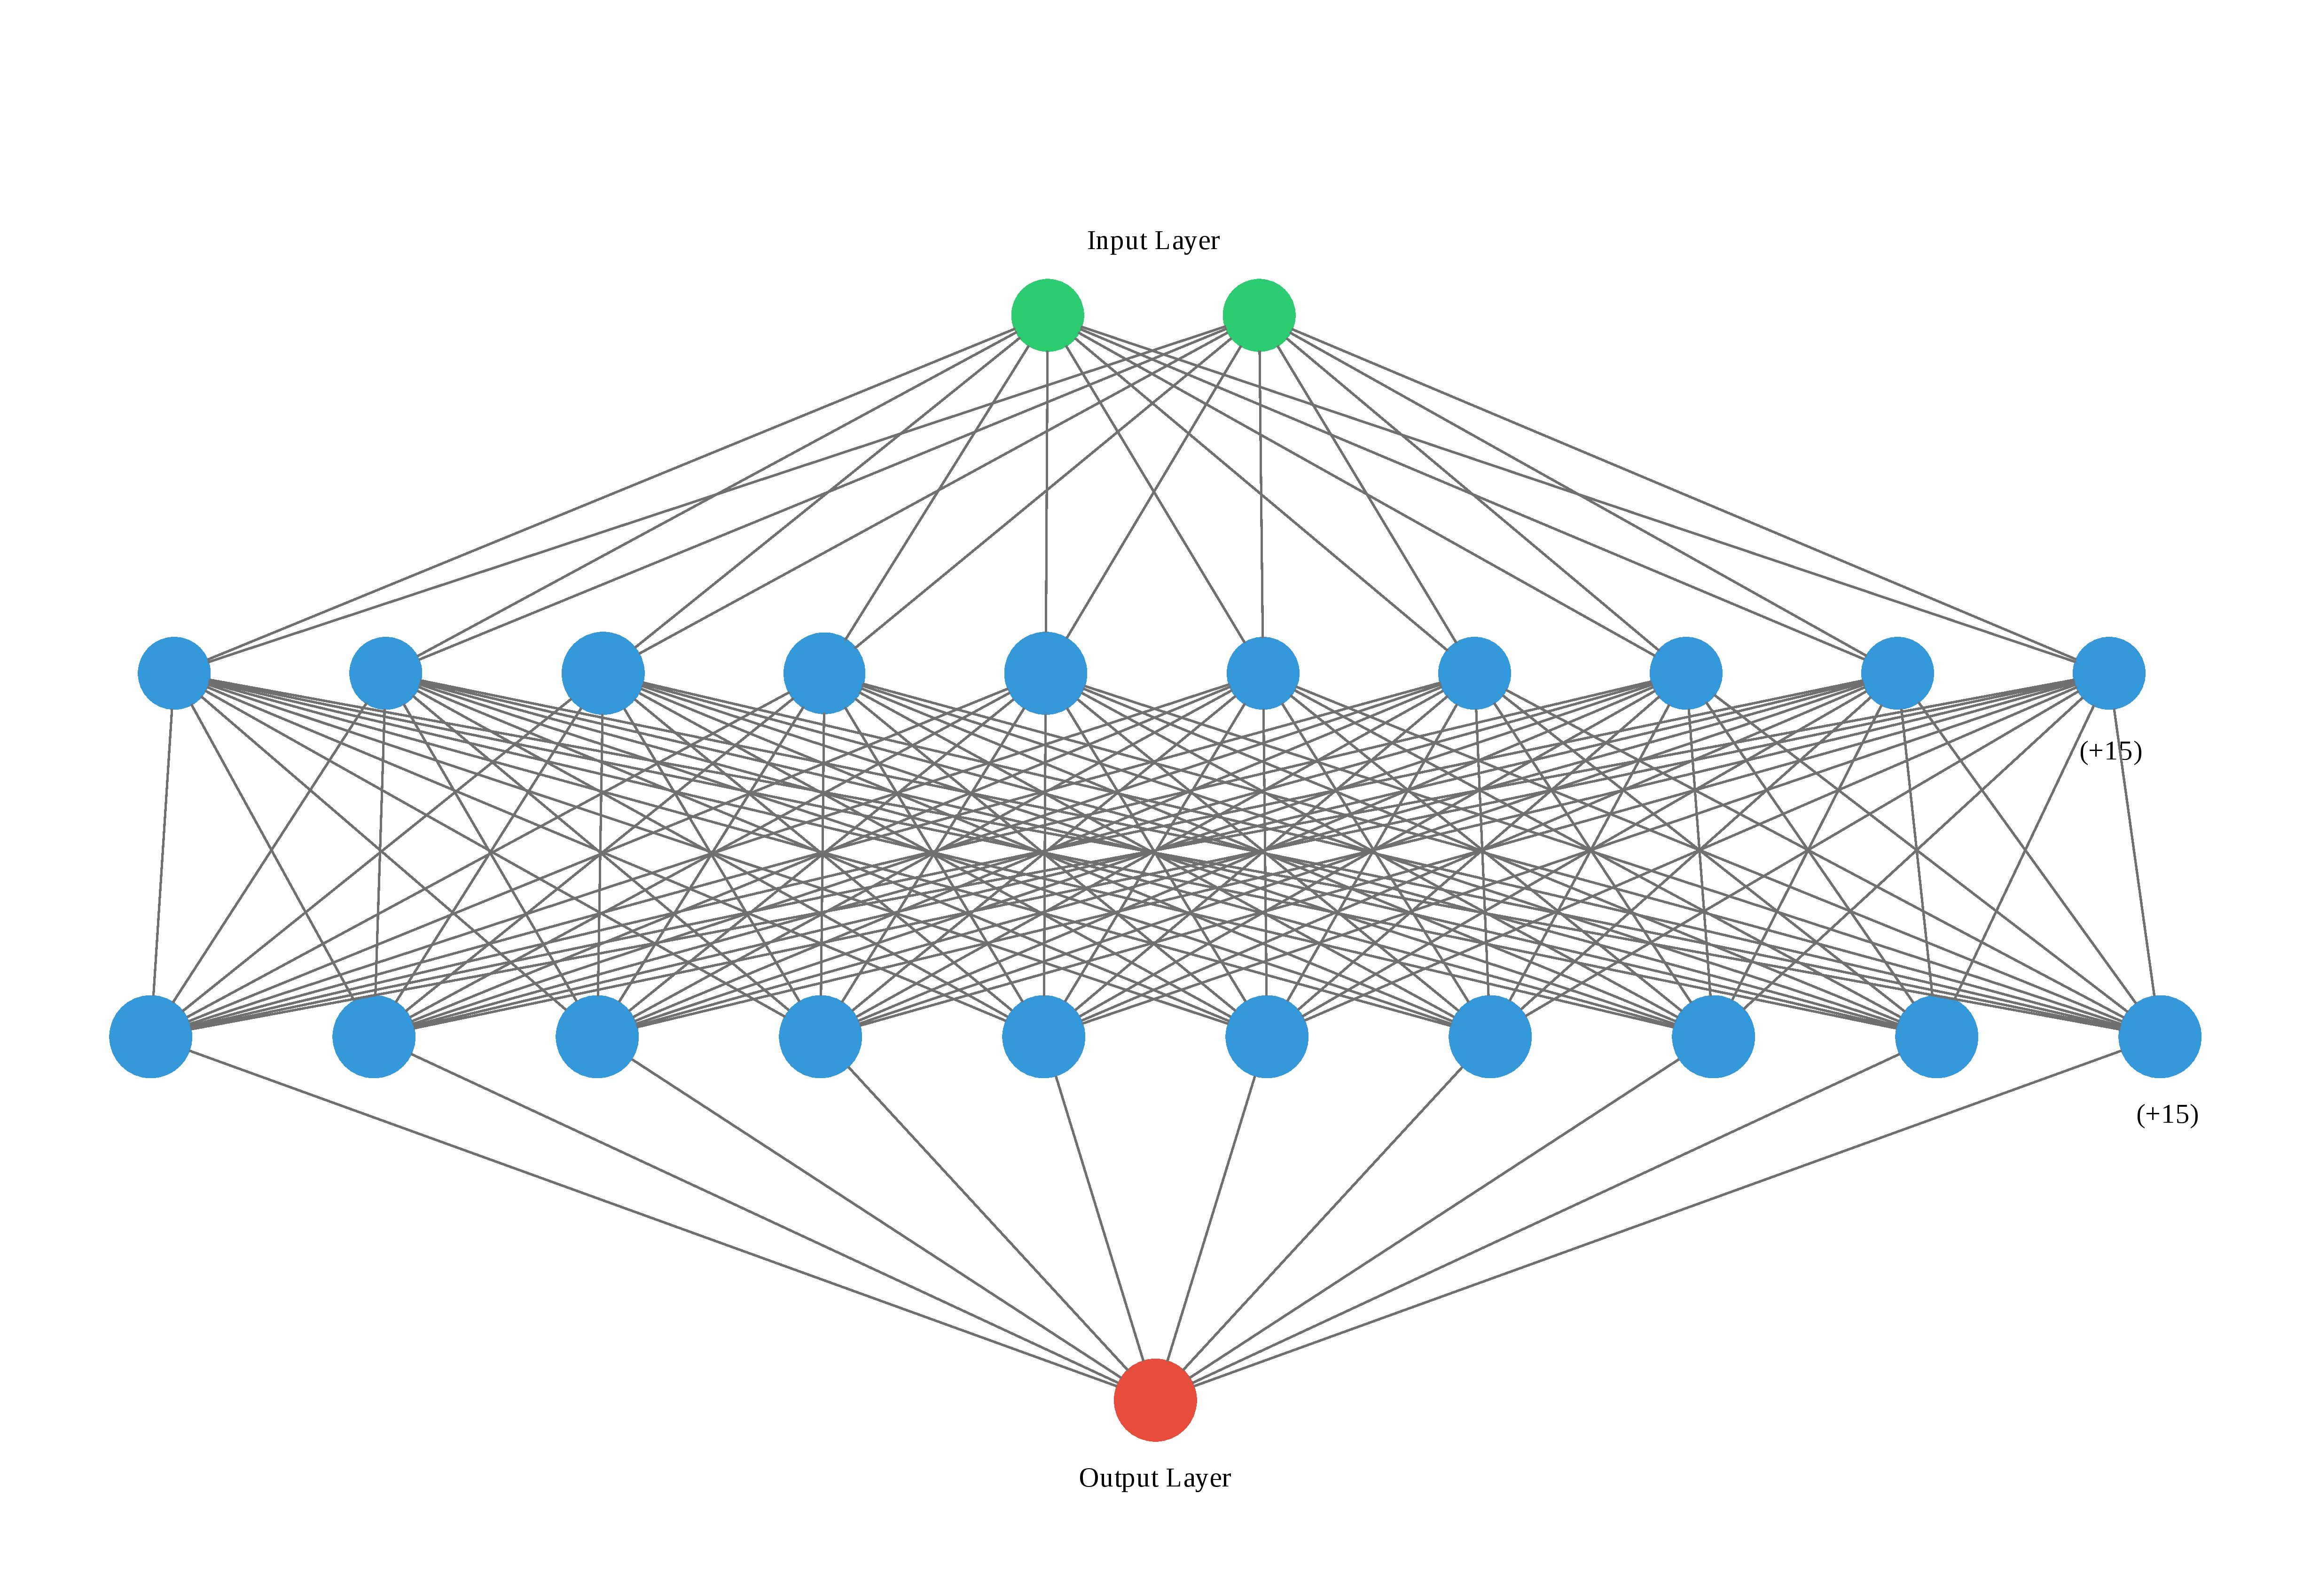
\includegraphics[width=0.8 \textwidth]{Images/1/DeepNetwork25.jpg}
    \caption{Two Hidden layers with 25 neurons each}
    \label{fig:figure23}
\end{figure}

\begin{figure}[H]
    \centering
    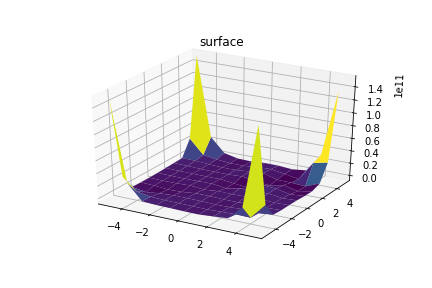
\includegraphics[width=0.8 \textwidth]{Images/1/PredictDeep.png}
    \caption{Approximating of $f(x)$ with $\mbox{MSE}$ 0.00}
    \label{fig:figure24}
\end{figure}

\subsection{Theorem}
Let $p(x)$ be a multivariate polynomial of degree $d$ and sparsity $c$, having monomials $q_1(x)$, $q_2(x)$ ... $q_c(x)$. Suppose that the nonlinearity $\sigma$ has nonzero Taylor coefficients up to degree $2d$. Then, we have
    \begin{itemize}
        \item $m_1 (p) \geq \frac{1}{c}$ $\max_j$ $m_1(q_j)$
        \item $m (p) \leq \sum_j m(q_j)$
    \end{itemize}
This theorem gives us the least upper bound for minimum number of neurons required for shallow network which means it can be at least maximum of minimum number of neurons required to estimate one monomial of that polynomial. It gives us an upper bound on the minimum number of neurons required for deep network which is just the sum of minimum number of neurons required to estimate each monomial with more layers.

% was testing on e thing
\section{Visual Proof for Neural Networks' universality}

The paper published in 1989 by Cybenko \cite{paper1989_1} which proved the universality of neural networks used sound mathematical arguments. In this section, we will present a visual proof for the universality of neural networks. In this proof, we will be using neural networks with two hidden layers\cite{website1}. Before we start with the proof, we need to how different parameters control the final value that is output from the neural network.

\subsection{Universality with one input and one output}
The output from the neuron is equal to $\sigma (\omega x + b ) $ where $\sigma(z)$ is the sigmoid function, $b$ is the bias, and $\omega$ is the weight. See Figure \ref{fig:figure2}. Increasing the value of the bias $b$ graph shifts to the left whereas decreasing the value of the bias $b$ shifts the graph to the right. On the other hand, $\omega$ controls the steepness of the curve.

\begin{figure}[H]
    \centering
    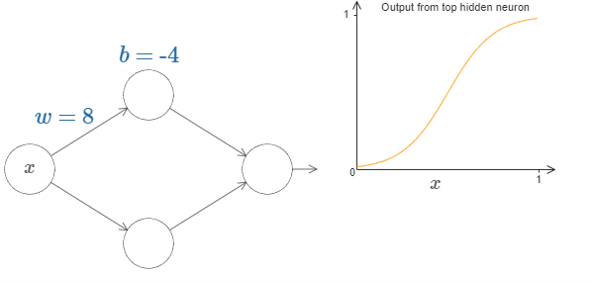
\includegraphics[width=0.8 \textwidth]{Images/2/1.png}
    \caption{Graph of the output from the top neuron in the hidden layer}
    \label{fig:figure2}
\end{figure}

If $\omega$ is assigned a very high value, then the output from the hidden layer will start to resemble a step function. See  Figure \ref{fig:figure3}. The reason for this approach is it that it is much easier to analyse the sum of step functions.

\begin{figure}[h!]
    \centering
    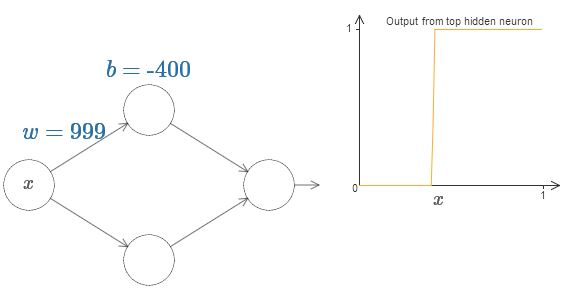
\includegraphics[width=0.8 \textwidth]{Images/2/2.png}
    \caption{Output from the top neuron in the hidden layer resembling the graph of a step function}
    \label{fig:figure3}
\end{figure}
The next thing that we will consider is how the values of $\omega$ and $b$ determine the position of the step. The position of the step is directly proportional to $b$ and inversely proportional to $\omega$. See Figure \ref{fig:figure4}.

\begin{figure}[H]
    \centering
    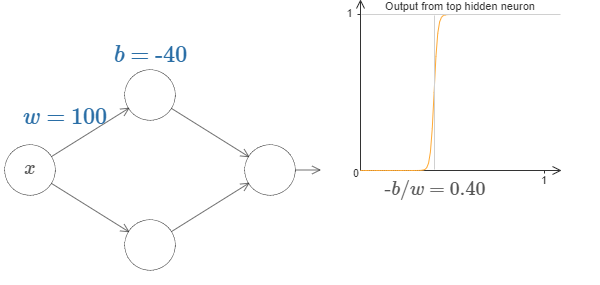
\includegraphics[width=0.8 \textwidth]{Images/2/3.png}
     \caption{The position of the step is directly proportional to $b$ and inversely proportional to $\omega$}
    \label{fig:figure4}
\end{figure}
Let  $s$ denote the position of the step. $ s = - \frac{b}{w} $. If we the value of $\omega$ is kept constant, we can represent each neuron using a single parameter $s$. In order, to change the position of step, we can then alter the value of $ b = -\omega s$. See Figure \ref{fig:figure5}.

\begin{figure}[H]
    \centering
    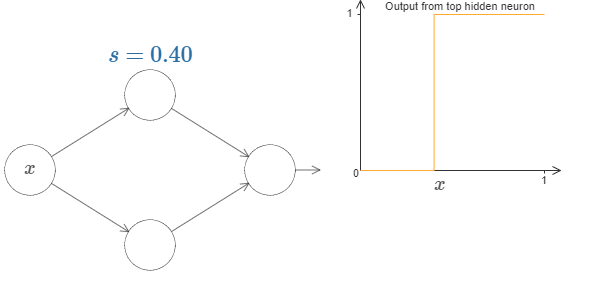
\includegraphics[width=0.8 \textwidth]{Images/2/4.png}
 
      \caption{$s = -\frac{b}{\omega}$}
    \label{fig:figure5}
\end{figure}

The weighted output from the hidden layer is equal to $a_1 \omega_1 + a_2 \omega_2 $ where $a_1$ and $a_2$ are outputs from the top and the bottom neurons in the hidden layer. For, example consider the graph in Figure \ref{fig:figure6}. From the graph, we can see that peaks occurs at the values $0.4$ and $0.6$ , which correspond to the values of $s_1$ and $s_2$. In addition to, the heights of the peak correspond to $0.6$ and $1.8$, which is the sum of $0.6$ and $1.2$.

\begin{figure}[h!]
    \centering
    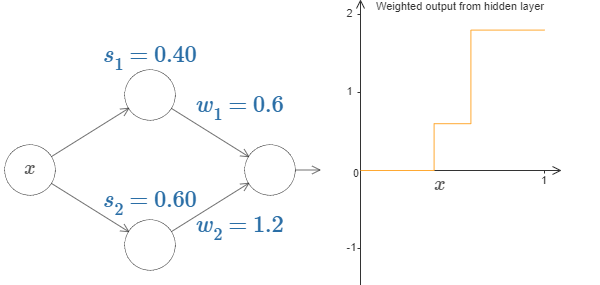
\includegraphics[width=0.7 \textwidth]{Images/2/5.png}
    \caption{The weighted output from the hidden layer}
    \label{fig:figure6}
\end{figure}
\newpage
 We can also generate bumps in the graph by using negative weights. See Figure \ref{fig:figure7} in which the value of $w_2 = - w_1$.

\begin{figure}[h!]
    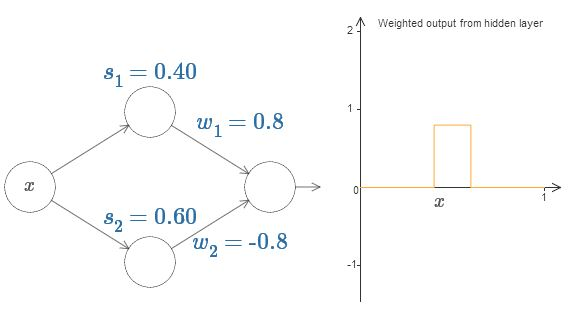
\includegraphics[width=0.8 \textwidth]{Images/2/6.png}
    \caption{$w_1 = - w_2$}
    \label{fig:figure7}
\end{figure}

In order to reduce, the overcrowding of the diagrams we can use an another parameter $h$ to describe each neuron.The parameter represents $h$ the height of the rectangle and value of  $ h =  w_1 =  - w_2$.

\begin{figure}[h!]
    \centering
    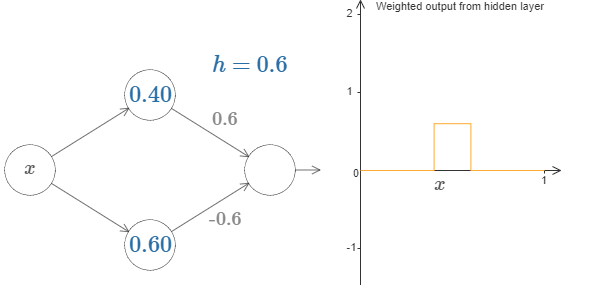
\includegraphics[width=0.8 \textwidth]{Images/2/10.png}
    \caption{$h = w_1 = -w_2$}
    \label{fig:figure8}
\end{figure}


In order to generate a graph with $N$ peaks, we can divide the interval into N sub-intervals and then use $N$ pairs of neurons to get peaks of any  desired height. As an example, consider the graph in Figure \ref{fig:figure9}. In to order generate, 5 peaks we used 10 neurons in the hidden layer.

\begin{figure}[h!]
    \centering
    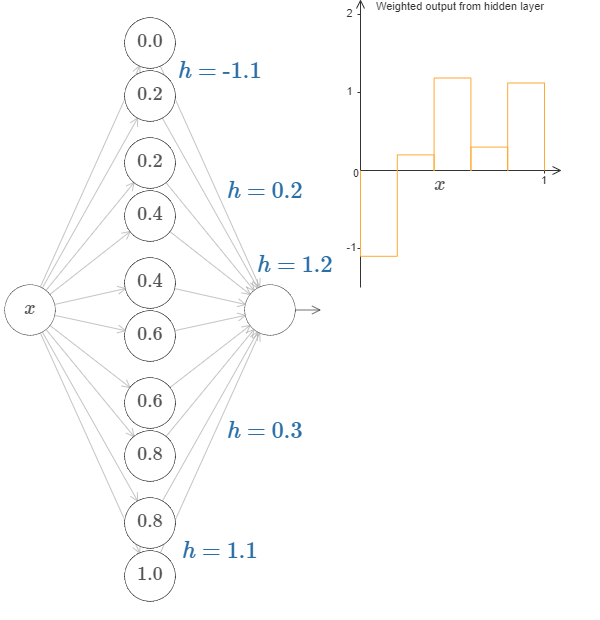
\includegraphics[width=0.8 \textwidth]{Images/2/8.png}
    \caption{$N$ = 5 Peaks}
    \label{fig:figure9}
\end{figure}

We have seen how different parameters control the output from the hidden layer, but in order to approximate $f(x)$ we some also need method to control the output from the output layer. One way to tackle this problem is that the output from the hidden layer is equal to $\sigma^-1 f(x)$. If we are able to do so, then the neural network can approximate the function $f(x)$. As an example, consider graph of $f(x)$ and $\sigma^{-1} f(x)$. Using 10 neurons, we can approximate $\sigma^{-1} f(x)$ with average deviation equal to 0.40. See Figures \ref{fig:figure10},\ref{fig:figure11},\ref{fig:figure12}



\begin{figure}[h!]

\centering
    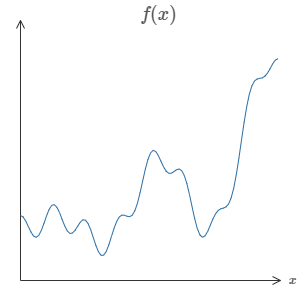
\includegraphics[width=0.4 \textwidth]{Images/2/22.png}
    \caption{Graph of the function $f(x)$}
    \label{fig:figure10}
\end{figure}

\newpage

\begin{figure}[h!]
\centering
    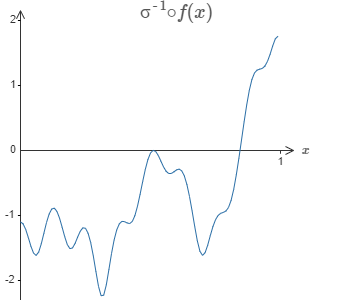
\includegraphics[width=0.4 \textwidth]{Images/2/9.png}
    \caption{Graph of the function $\sigma^{-1} f(x)$}
    \label{fig:figure11}
\end{figure}


\begin{figure}[h!]
    \centering
    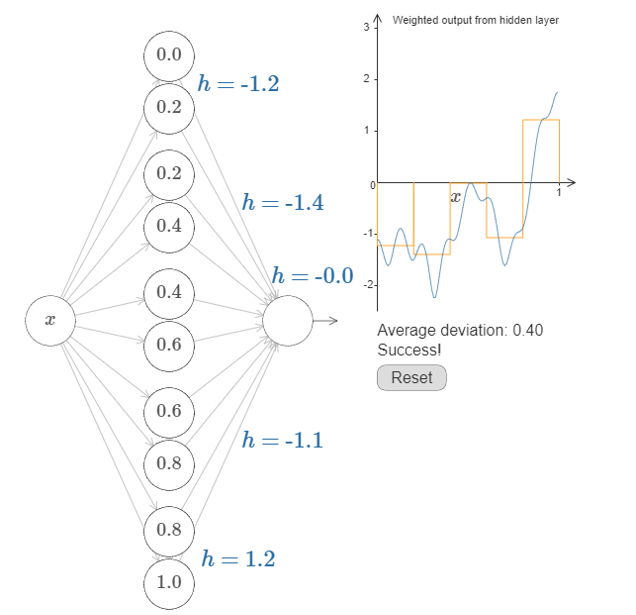
\includegraphics[width=0.8 \textwidth]{Images/2/7.png}
    \caption{Approximating the function $\sigma^{-1} f(x)$ with 10 Neurons}
    \label{fig:figure12}
\end{figure}

\newpage

\subsection{Two Input Variables}
The ideas that we learned for one input neural networks can be extended easily to neural networks with two input variables. 
Let's focus on the input individually before looking at the combined output. Setting $w_2 = 0$ means that input y will not have an effect on the output of the hidden layer and setting $w_1=0$ means that x will not have an effect on the output of the hidden layer. The affect of changing values of $\omega$ and $b$ on the output is same as a neural network with one input variable. See Figure \ref{fig:figure13}
\begin{figure}[H]
    \centering
    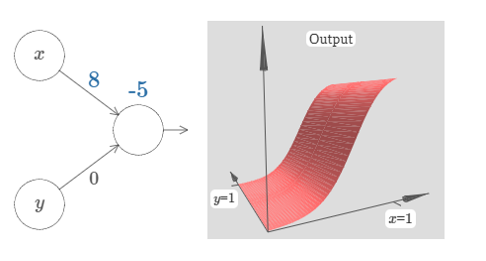
\includegraphics[width=0.5 \textwidth]{Images/2/11.png}
    \caption{Output from the top neuron in the hidden layer}
    \label{fig:figure13}
\end{figure}
Since the step function is in three dimensions, we will x step position , $s_x = -\frac{b}{\omega_1}$ and y-step position $s_y = -\frac{b}{\omega_2}$. See the Figure \ref{fig:figure14}

\begin{figure}[H]
    \centering
     \begin{subfigure}[b]{0.5\textwidth}
     \centering
         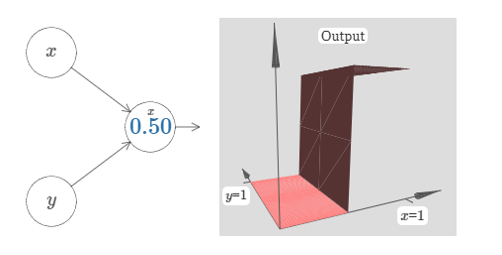
\includegraphics[width=\textwidth]{Images/2/12.png}
         \caption{$s_1=-\frac{b}{\omega_1}$}
         \label{fig:y equals x}
     \end{subfigure}
     \hfill
     
     \begin{subfigure}[b]{0.5\textwidth}
     \centering
         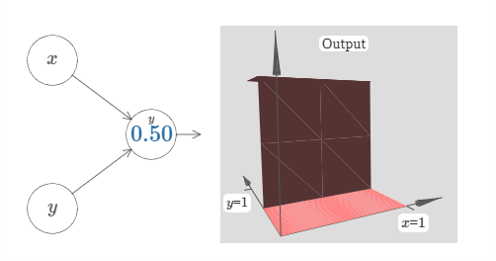
\includegraphics[width = \textwidth]{Images/2/13.png}
         \caption{$s_2=-\frac{b}{\omega_2}$}
         \label{fig:three sin x}
     \end{subfigure}
     \caption{Step Positions $s_1,s_2$}
    \label{fig:figure14}
\end{figure}
\newpage
\begin{figure}
    \centering
     \begin{subfigure}[b]{0.7\textwidth}
     \centering
         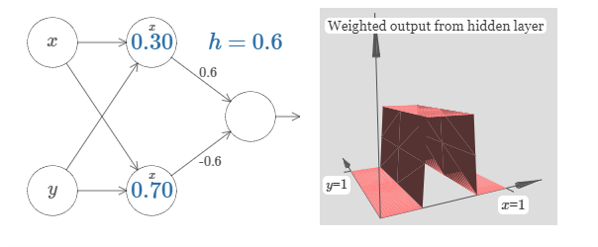
\includegraphics[width=\textwidth]{Images/2/14.png}
         \caption{Weighted Output in the x direction}
         \label{fig:x}
     \end{subfigure}
     \hfill
     \begin{subfigure}[b]{0.7\textwidth}
     \centering
         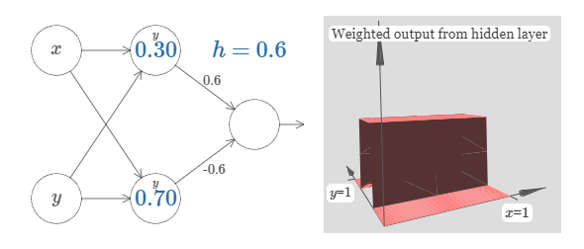
\includegraphics[width=\textwidth]{Images/2/15.png}
         \caption{Weighted Output in the y direction}
         \label{fig:y}
     \end{subfigure}
     \begin{subfigure}[b]{0.7\textwidth}
     \centering
         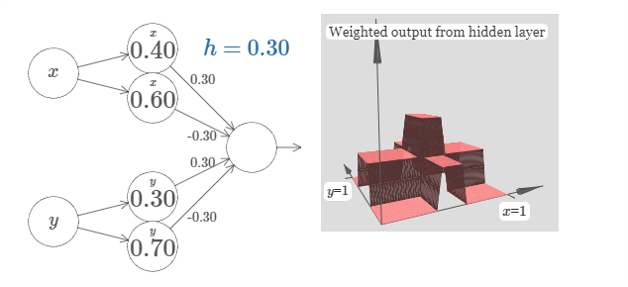
\includegraphics[width=\textwidth]{Images/2/16.png}
         \caption{Weighted Output in both x \& y direction}
         \label{fig:xy}
     \end{subfigure}
     \caption{Weighted Output from the hidden layer}
    \label{fig:figure15}
\end{figure}

In case of one input variable, we generated rectangles but in case of two input variables we will be generating tower functions. However, first we will create step functions in the $x$-direction and $y$-direction. See Figure \ref{fig:x}, \ref{fig:y}. 
\newpage
If $ b = -\frac{3}{2}h$, then the output of the graph will resemble a tower function. See Figure \ref{fig:figure16}.
\begin{figure}[h!]
    \centering
    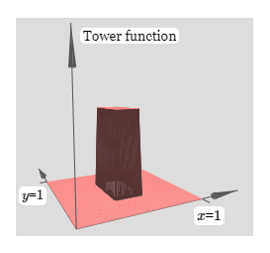
\includegraphics[width=0.5 \textwidth]{Images/2/17.png}
    \caption{Tower Function}
    \label{fig:figure16}
\end{figure}
In Figure \ref{fig:xy}, we can see that the output of the function is similar to a tower, but we still need to modify the values of $h$ and $b$. See Figure \ref{fig:figure16}. 
We can combine the output of two networks in the second hidden layer to generate two multiple tower functions. 
\begin{figure}[h!]
    \centering
    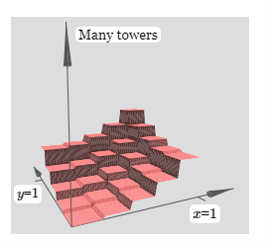
\includegraphics[width=0.5 \textwidth]{Images/2/18.png}
    \caption{Tower Function}
    \label{fig:figure17}
\end{figure}
This idea can be further extended and we can combine multiple networks to generate multiple towers. Using large number of towers allows us to better approximate the function.
\begin{figure}[h!]
    \centering
    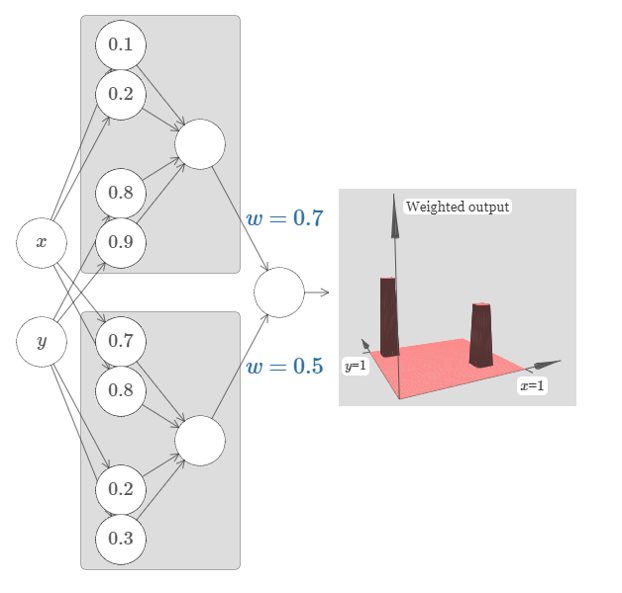
\includegraphics[width=0.5 \textwidth]{Images/2/19.png}
    \caption{Many towers}
    \label{fig:figure18}
\end{figure}
\newpage
\subsection{Three Input Variables}
The ideas that we learned for two Input variables can be extend to neural networks with three input variables . In Figure \ref{fig:figure19}, with three input variables, we will be generating tower functions in four dimensions.
\begin{figure}[h!]
    \centering
    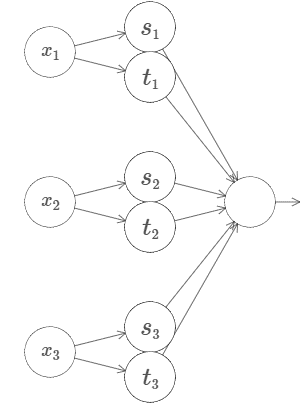
\includegraphics[width=0.3 \textwidth]{Images/2/21.png}
    \caption{Neural Network with three inputs}
    \label{fig:figure19}
\end{figure}
\newpage

\section{Conclusion}
We have showed and analyzed different theorems which talked about the possibility of neural networks approximating functions which tells us that neural networks are a class of universal approximators. We also showed some results where using deep networks and adding more layers required us less neurons in total which became very efficient with increasing number of inputs because minimum number of neurons in shallow network was growing exponentially. We also showed the bounds on minimum number of neurons and visualized some functions and their approximations with neural networks with different parameters.

\bibliography{references}
\bibliographystyle{plain}

\end{document}
